\section {Вычисление асимптотических результатов}
В данной главе будет рассмотрен метод вычисления коэффициента вариации длин интервалов между моментами поступления заявок входящего потока. Помимо этого, будет предложен метод вычисления вероятностей при помощи дискретного преобразования Фурье.
\subsection{Использование дискретного преобразования Фурье}
Ранее при вычислении распределения вероятностей числа обслуженных заявок с помощью асимптотических формул использовалось обратное преобразование Фурье для дискретных случайных величин (\ref{distr},\ref{distr2}). Однако полученные формулы подходят лишь для точечных проверок из-за сложности вычисления. В случае с двумерным распределением вероятностей, процесс подсчета плоскость размером 10 на 10 точек может занимать около минуты. Чтобы решить проблему чрезвычайно долгого вычисления было принято решение использовать дискретное преобразование Фурье с заданной точностью \cite{nussbaumer1981fast,bergland1969guided}. Особенность данного метода заключается в выборе такого шага дискретизации $\delta$, чтобы в результате преобразования основная часть результирующего распределения не повторялась и совпадала с искомым. Шаг дискретизации был выбран согласно интервалу интегрирования и вычисляется следующим образом
\begin{equation*}
	\delta = \frac{2\pi}{n},
\end{equation*}
где $n$ --- длина результирующего вектора. Таким образом, для корректного преобразования требуется подобрать длину вектора таким образом, чтобы оно охватывало часть распределения в районе математического ожидания в диапазоне значения дисперсии. 

Были рассмотрены одномерный и двумерный случаи преобразования
\begin{equation*}
	B_n =\frac{1}{\sqrt{n}} \sum_{k=0}^{N-1} W_k \cdot e^{-2\pi\j (n/N)k}
\end{equation*}
\begin{equation*}
	B_{n,m} =\frac{1}{\sqrt{nm}} \sum_{k=0}^{N-1}\sum_{h=0}^{M-1} W_{k,h} \cdot e^{-2\pi\j (n/N)k -2\pi\j(m/M)h} 
\end{equation*}
Была написана реализация на языке Python для одномерного и двумерного случаев. В качестве вспомогательной библиотеки для операций над векторами использовалась numpy \cite{harris2020array}.
\lstset{language=Python,
	basicstyle=\linespread{0.8}\ttfamily,
	caption={Реализация ДПФ на Python}
}
\begin{lstlisting}
import numpy as np

def icfft(n,vector):
	d = np.zeros(n,dtype=complex)
	for j in range(0,n-1):
		for k in range(0,n-1):
			d[j] += vector[k]*np.exp(-2*np.pi*1j*(j/n)*k)
		d[j] *= 1/np.sqrt(n)
	return d

def icfft2(n,m,matrix):
	d = np.zeros((n,m),dtype=complex)
	for j in range(0,n-1):
		for i in range(0,m-1):
			for k in range(0,n-1):
				for h in range(0,m-1):
					d[j][i] += matrix[k][h]*np.exp(-2*np.pi*1j*(j/n)*k - 2*np.pi*1j*(i/m)*h)
			d[j][i] *= 1/np.sqrt(n*m)
	return d
\end{lstlisting}

\lstset{language=Python,
	basicstyle=\linespread{0.8}\ttfamily,
	caption={Вычисление ДПФ на Python}
}
\begin{lstlisting}
length =30
iii = list(range(0,length-1))
delta = (2*np.pi)/length
res = []
for i in iii:
res.append(complex(s.SFF(-np.pi + i * delta,10)))
ifft = [abs(n)/np.sqrt(length) for n in icfft(length,res)]
\end{lstlisting}
На рисунке \ref{ifft_plot_test} видно, что полученное преобразование (IFFT) полностью совпадает с результатом вычисления при помощи интегрирования (SDST)
\begin{figure}[H]
	\centering
	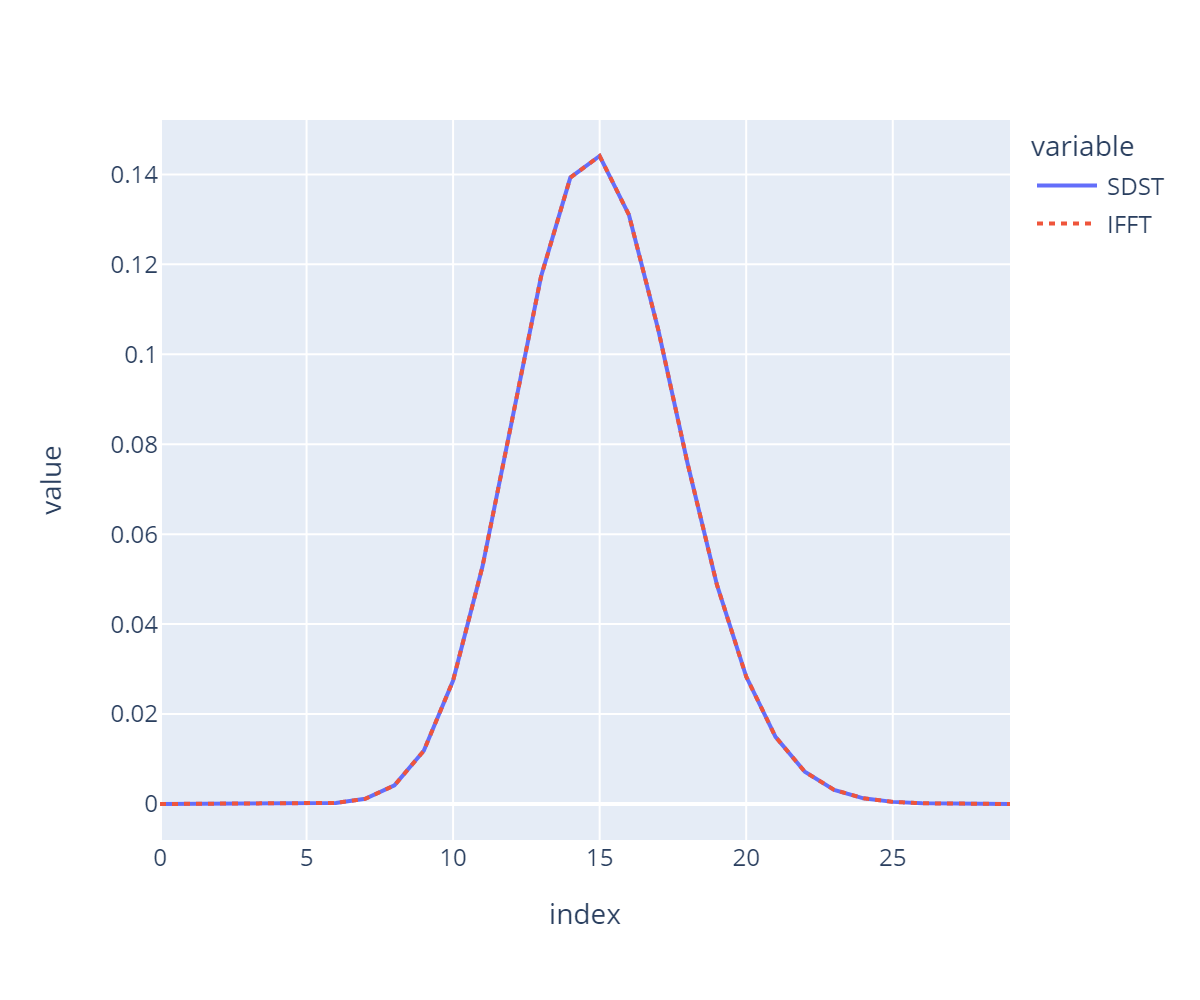
\includegraphics[scale=0.8,width=\textwidth]{ifft_plot_test.png}
	\caption{Сравнение распределений вероятностей, полученных с помощью интегрирования и ДПФ}
	\label{ifft_plot_test}
\end{figure}
Для проверки скорости работы данного подхода к вычислению был проведен ряд тестов (150 запусков для одномерного и двумрного случая) со сравнением скорости работы алгоритмов и точности получаемого распределения при помощи расстояния Колмогорова
\begin{equation*}
	\Delta = \underset{0 < i < \infty}{max}\bigg\rvert \sum_{v=0}^{i} (P_0(v) - P_1(v))\bigg\rvert.
\end{equation*}
Были получены следующие результаты:
\begin{itemize}
	\item Для одномерного случая в среднем ДПФ быстрее интегрирования в 411.717 раза, среднее расстояние Колмогорова --- 4.164439016729942e-06.
	\item Для двумерного случая в среднем ДПФ быстрее интегрирования в 901.184 раза, среднее расстояние Колмогорова --- 2.157044454159e-06.
\end{itemize}
Так, можно заключить, что дискретное преобразование Фурье не проигрывает в точности и в то же время существенно быстрее, что является важным результатом для последующей работы.
\subsection{Вычисление коэффициента вариации MMPP}
В данной работе одним из объектов изучения является вариация длин интервалов между моментами поступления заявок MMPP.

Согласно \cite{вишневский2018стохастические}, вариация длин интервалов между моментами поступления заявок MMPP вычисляется как
\begin{equation}
	Var = \frac{\sqrt{v}}{Lg^{-1}},
\end{equation}
где $v$ --- дисперсия длин интервалов между моментами поступления групп запросов и рассчитывается как
\begin{equation}
	v = \frac{2Lg\cdot r \cdot (-D0)^{-1} \cdot E -1}{Lg^2},
\end{equation}
где вектор--строка $r$ --- стационарное распределение вероятностей процесса\\$\{k(t),n(t)\}$, $E$ --- единичный вектор--столбец размерности N, $Lg$ -- интенсивность входящего потока
\begin{equation} \label{eq_lg}
	Lg = r\cdot \Lambda \cdot E,
\end{equation}
\begin{equation*}
	D0 = Q - \Lambda - Q\cdot D,
\end{equation*}
где $D$ --- матрица, содержащая вероятности наступления события в потоке при смене его состояния.
\clearpage
